\chapter{拉格朗日力学}\label{ch:b3:lagrangian-mechanics}

试写出双摆的牛顿定律：两个张力事先都未知，
且每时每刻方向都在变化，
还要解四个标量方程，才能求出两个角度如何演化。
再对套在旋转圆环上的珠子、一串耦合弹簧、
一只机器人手臂做同样的分析。维系系统整体的力——杆、
导轨、铰链——不做功，但牛顿方法迫使我们
在每一步计算中都带着它们。本章介绍拉格朗日于 1788 年发表的重新表述：
用真正能够变化的少数几个坐标描述系统，
写出一个单一的函数
$L = E_k - E_p$，再用一个统一的方法即可在任意坐标下得出运动方程，
所有杆和导轨都已被消去。更妙的是，
新的表述揭示了牛顿表述所隐藏的东西：$L$ 的每一个对称性
都给出一个守恒量——空间均匀性对应动量，
时间均匀性对应能量——这一结论由埃米·诺特得出，
它已成为远超力学范畴的物理学组织原则。

\section{从力到坐标}

\begin{definition}[约束、自由度、广义坐标]\label{def:b3:lagrangian-mechanics:coordinates}
\index{约束}\index{自由度}\index{广义坐标}
\emph{约束}是加在系统位置上的几何条件——
珠子始终套在它的导线上，摆杆长度保持不变，车轴上的两个车轮同步转动。
若一个约束可用坐标（必要时还包括时间）之间的方程
$f(\vect r_1, \dots, \vect r_N, t) = 0$ 表示，
则称该约束为\emph{完整约束}。
构型仍可能变化的独立方式的数目
称为\emph{自由度} $n$；能完全确定构型的任一组 $n$ 个独立量
$q_1, \dots, q_n$ 称为一组\emph{广义坐标}——它们可以是角度、长度，
或任何方便的混合量。
其时间导数 $\dot q_1, \dots, \dot q_n$
称为\emph{广义速度}\index{广义速度}。
\end{definition}

\begin{example}[自由度计数]\label{ex:b3:lagrangian-mechanics:counting}
桌面上的一个点：$n = 2$。长度固定的平面单摆：一个角度，$n = 1$。
双摆：两个角度，$n = 1 + 1 = 2$。固定在刚性圆环上的珠子：一个角度，$n = 1$——
即使圆环本身被强制转动，所加的转动也不增加自由度。
空间中自由的刚体：其质心的三个坐标
加上三个角度，$n = 6$。
$N$ 个自由分子（质点）组成的气体：$n = 3N$。
每一个完整约束消去一个自由度：用杆相连的两个质点
有 $3 + 3 - 1 = 5$。
\end{example}

\begin{omfigure}
\begin{tikzpicture}[font=\small, >=Stealth]
  % (a) plane pendulum
  \begin{scope}
    \draw[thick] (-1,0) -- (1,0);
    \foreach \i in {-0.8,-0.5,-0.2,0.1,0.4,0.7} \draw (\i,0) -- (\i+0.18,0.16);
    \fill (0,0) circle (1.5pt);
    \draw[dashed] (0,0) -- (0,-2.2);
    \draw[thick] (0,0) -- (-55:2.1);
    \fill[omDef] (-55:2.1) circle (3pt);
    \draw[->] (0,-1.0) arc (-90:-55:1.0);
    \node at (-72:1.35) {$\theta$};
    \node at (-55:2.5) {$m$};
    \node at ($(-55:1.35)+(0.28,0.12)$) {$\ell$};
    \node at (0,-2.9) {一个坐标：$\theta$};
  \end{scope}
  % (b) bead on rotating hoop
  \begin{scope}[xshift=6.2cm]
    \coordinate (C) at (0,-2.35);
    \draw[thick] (C) circle (1.55);
    \draw[dashed] (0,-0.3) -- (0,-4.6);
    \draw[->, thick] (0.35,-0.15) arc (20:160:0.37);
    \node at (0,0.25) {$\omega$};
    \fill (C) circle (1pt);
    \draw (C) -- ++(-50:1.55);
    \fill[omDef] ($(C)+(-50:1.55)$) circle (3pt);
    \draw[->] ($(C)+(0,-0.85)$) arc (-90:-50:0.85);
    \node at ($(C)+(-70:1.18)$) {$\theta$};
    \node at ($(C)+(-38:2.0)$) {$m$};
    \draw (C) -- ++(135:1.55);
    \node at (-1.35,-1.35) {$R$};
    \node at (0,-4.95) {一个坐标：$\theta$};
  \end{scope}
  % (c) double pendulum
  \begin{scope}[xshift=11.4cm]
    \draw[thick] (-0.9,0) -- (0.9,0);
    \foreach \i in {-0.7,-0.4,-0.1,0.2,0.5} \draw (\i,0) -- (\i+0.18,0.16);
    \fill (0,0) circle (1.5pt);
    \draw[dashed] (0,0) -- (0,-1.7);
    \draw[thick] (0,0) -- (-65:1.5) coordinate (m1);
    \fill[omDef] (m1) circle (2.6pt);
    \draw[dashed] (m1) -- ++(0,-1.5);
    \draw[thick] (m1) -- ++(-40:1.5) coordinate (m2);
    \fill[omThm] (m2) circle (2.6pt);
    \draw[->] (0,-0.8) arc (-90:-65:0.8);
    \node at (-80:1.1) {$\theta_1$};
    \draw[->] ($(m1)+(0,-0.75)$) arc (-90:-40:0.75);
    \node at ($(m1)+(-68:1.05)$) {$\theta_2$};
    \node at (0.3,-3.4) {两个坐标：$\theta_1, \theta_2$};
  \end{scope}
\end{tikzpicture}

{\small 广义坐标：每个系统都由真正能够变化的
角度描述，而不是由其质点的笛卡儿坐标描述。
杆的张力和圆环的法向力从不出现。}
\end{omfigure}

\section{最小作用量原理}

\begin{definition}[拉格朗日量与作用量]\label{def:b3:lagrangian-mechanics:action}
\index{拉格朗日量}\index{作用量}
若一个力学系统的力由势能 $E_p$ 导出，则其\emph{拉格朗日量}
是坐标、速度以及（可能）时间的函数，
记为
\[
L(q, \dot q, t) = E_k - E_p ,
\]
即动能\emph{减去}势能，两者均用
广义坐标表示。对于设想运动 $q(t)$ 的\emph{作用量}，
在端点固定为 $q(t_1)$ 和 $q(t_2)$ 的情形下，其值为
\[
S[q] = \int_{t_1}^{t_2} L\big(q(t), \dot q(t), t\big)\,\dd t .
\]
$S$ 是一个\emph{泛函}：它作用于整条路径，
返回一个数，单位为焦耳·秒——即普朗克常量的单位。
\end{definition}

\begin{theorem}[哈密顿原理与欧拉–拉格朗日方程]\label{thm:b3:lagrangian-mechanics:euler-lagrange}
\index{哈密顿原理}\index{欧拉–拉格朗日方程}\index{最小作用量}
在所有可能的、连接相同两端点且用时相同的运动中，
实际运动是使作用量
\emph{驻定}（\emph{哈密顿原理}，或称
\emph{最小作用量}原理）。等价地，运动
满足\emph{欧拉–拉格朗日方程}：
\[
\frac{\dd}{\dd t}\frac{\partial L}{\partial\dot q_i}
 - \frac{\partial L}{\partial q_i} = 0 ,
\qquad i = 1, \dots, n :
\]
每个自由度对应一个二阶方程，
无论选取何种坐标。
\end{theorem}

\begin{proof}
作路径变形：$q_i(t) \to q_i(t) + \delta q_i(t)$，满足
$\delta q_i(t_1) = \delta q_i(t_2) = 0$。一阶近似下，
\[
\delta S = \int_{t_1}^{t_2}\sum_i\Big(
  \frac{\partial L}{\partial q_i}\,\delta q_i
 + \frac{\partial L}{\partial\dot q_i}\,\delta\dot q_i\Big)\dd t
 = \int_{t_1}^{t_2}\sum_i\Big(
  \frac{\partial L}{\partial q_i}
 - \frac{\dd}{\dd t}\frac{\partial L}{\partial\dot q_i}\Big)\delta q_i\,\dd t ,
\]
对第二项作分部积分（$\delta\dot q_i =
\dd(\delta q_i)/\dd t$），并舍去边界项，
它在固定端点处为零。若对\emph{任一}变形均有 $\delta S = 0$，
则括号内的量须在每一时刻、对每个 $i$ 均为零——若它
在某处为正，则集中在该处的凸起 $\delta q_i$ 将给出
$\delta S \neq 0$。逆命题可由同一式子直接读出。
\end{proof}

\begin{omfigure}
\begin{tikzpicture}[font=\small, >=Stealth]
  \draw[->] (0,0) -- (7.6,0) node[right] {$t$};
  \draw[->] (0,0) -- (0,3.4) node[above] {$q$};
  \fill (0.8,0.7) circle (2pt) node[below left] {$q(t_1)$};
  \fill (6.8,2.3) circle (2pt) node[above right] {$q(t_2)$};
  \draw[omDef, very thick] (0.8,0.7) .. controls (2.6,2.6) and (5.0,1.4) .. (6.8,2.3);
  \draw[omExo, dashed] (0.8,0.7) .. controls (2.2,0.6) and (5.4,0.9) .. (6.8,2.3);
  \draw[omExo, dashed] (0.8,0.7) .. controls (3.0,3.6) and (5.2,2.9) .. (6.8,2.3);
  \node[omDef] at (1.9,3.35) {实际路径};
  \draw[->, omDef] (2.25,3.15) -- (2.85,2.3);
  \node[omExo] at (3.4,0.42) {变形路径};
  \draw[<->] (4.1,1.62) -- (4.1,2.62);
  \node at (4.55,2.15) {$\delta q$};
\end{tikzpicture}

{\small 哈密顿原理：在所有端点与历时均相同的路径中，
实际路径使 $S = \int L\,\dd t$ 驻定——
一阶变形 $\delta q$ 仅在二阶上改变 $S$。}
\end{omfigure}

\begin{proposition}[牛顿定律的再现]\label{prop:b3:lagrangian-mechanics:newton}
对直角坐标系中的质点，$L = \tfrac12 m(\dot x^2 +
\dot y^2 + \dot z^2) - E_p(x,y,z)$，欧拉–拉格朗日方程
写成 $m\ddot x = -\partial E_p/\partial x$，对 $y$、$z$ 同理：
恰为 $m\vect a = \vect F$。拉格朗日力学与牛顿力学
在两者均适用之处结论一致；新形式
在坐标变换下依然成立，牛顿的分量方程则不然。
\end{proposition}

\begin{proof}
$\partial L/\partial\dot x = m\dot x$, $\partial L/\partial x =
-\partial E_p/\partial x$；欧拉–拉格朗日方程为
$\dd(m\dot x)/\dd t + \partial E_p/\partial x = 0$。
\end{proof}

\begin{remark}[约束力为何消失]\label{rem:b3:lagrangian-mechanics:constraints}
杆中的张力、导轨的法向力，
与约束允许的任一位移都垂直，它们在任何与约束相容的运动中都不做功。
由于作用量仅由在这类运动上取值的能量构成，
这些力从不进入 $L$
——这正是本方法的实用“奇迹”。一般性论证
（达朗贝尔虚功原理）在本阶段不加证明地承认；
对本书的每个体系，下述方法都可直接与牛顿定律比对，
正如\cref{prop:b3:lagrangian-mechanics:newton}已开始做的那样。
若还需要约束力本身——杆会不会断？
——此时仅对该力回到牛顿定律，
并利用已知的运动求解。
\end{remark}

\begin{method}[拉格朗日方法步骤]\label{met:b3:lagrangian-mechanics:recipe}
（1）数出自由度，选取坐标 $q_i$——
转动用角度，沿导轨用横坐标。（2）
将位置写为 $\vect r(q_i, t)$，求导得速度，并写出
$E_k$；写出 $E_p$。（3）$L = E_k - E_p$，略去任意
可加常数。（4）每个坐标对应一个欧拉–拉格朗日方程。（5）求解之前，
先收集守恒量：循环坐标
（\cref{def:b3:lagrangian-mechanics:momentum}）与能量函数
（\cref{prop:b3:lagrangian-mechanics:energy}）。（6）检验极限：小
角度、关闭转动、已知特例。
\end{method}

\begin{example}[单摆：三行推导]\label{ex:b3:lagrangian-mechanics:pendulum}
只有一个坐标 $\theta$；$\vect v = \ell\dot\theta\,\vect e_\theta$，故
$E_k = \tfrac12 m\ell^2\dot\theta^2$，$E_p = -mg\ell\cos\theta$。
于是 $L = \tfrac12 m\ell^2\dot\theta^2 + mg\ell\cos\theta$，并得
$\dd(m\ell^2\dot\theta)/\dd t = -mg\ell\sin\theta$：
\[
\ddot\theta = -\frac{g}{\ell}\sin\theta ,
\]
这正是本科一年级分册中由重力的力矩得出的方程
——全程未提及张力。
\end{example}

\begin{example}[旋转圆环上的小珠]\label{ex:b3:lagrangian-mechanics:hoop}
质量为 $m$ 的小珠沿半径为 $R$ 的竖直圆环滑动，
该圆环被迫以恒定角速度 $\omega$ 绕其竖直直径转动
（见\cref{ex:b3:lagrangian-mechanics:counting}）。取一个坐标，即
自底部起算的极角 $\theta$。小珠的速度有
沿圆环的分量 $R\dot\theta$，以及由所施加转动引起的分量 $\omega R\sin\theta$，
其方向垂直于圆环：
\[
L = \tfrac12 mR^2\dot\theta^2 + \tfrac12 m\omega^2R^2\sin^2\theta
 + mgR\cos\theta ,
\qquad
mR^2\ddot\theta = m\omega^2R^2\sin\theta\cos\theta - mgR\sin\theta .
\]
平衡位置满足 $\ddot\theta = 0$：底部 $\theta = 0$（以及
顶部，总是不稳定的），以及当 $\omega^2 > g/R$ 时新增一对
平衡点 $\cos\theta_{\text{平衡}} = g/\omega^2R$。将方程写为
$mR^2\ddot\theta = -\dd U_{\text{有效}}/\dd\theta$，其中
引入\emph{有效势能}\index{有效势能}
\[
U_{\text{有效}}(\theta) = -mgR\cos\theta
 - \tfrac12 m\omega^2R^2\sin^2\theta
\]
使几何关系一目了然：低于临界角速率
$\omega_{\text{临界}} = \sqrt{g/R}$，底部为势阱；超过它后，
底部变为峰顶，小珠停在斜坡上，
圆环转得越快，小珠爬得越高——这正是离心
调速器的原理，它曾用于调节蒸汽机。
\end{example}

\begin{omfigure}
\begin{tikzpicture}
  \begin{axis}[omaxis, axis x line=bottom, axis y line=left,
    width=11.4cm, height=5.6cm, xmin=-180, xmax=180,
    ymin=-1.65, ymax=1.2, xlabel={$\theta$（度）},
    xlabel style={at={(axis description cs:0.5,-0.1)}, anchor=north},
    ylabel={$U_{\text{有效}}/mgR$}, xtick={-180,-90,0,90,180}, ytick=\empty,
    clip=false,
    legend style={font=\scriptsize, at={(0.5,-0.32)}, anchor=north,
      draw=none, fill=none, legend columns=2}]
    \addplot[omDef, thick, domain=-180:180, samples=90]
      {-cos(x) - 0.25*sin(x)^2};
    \addlegendentry{$\omega^2 = g/2R$（慢）：$\theta = 0$ 处为势阱}
    \addplot[omThm, thick, domain=-180:180, samples=90]
      {-cos(x) - 1.0*sin(x)^2};
    \addlegendentry{$\omega^2 = 2g/R$（快）：$\pm 60^\circ$ 处为势阱}
    \fill[omThm] (axis cs:60,-1.25) circle (1.8pt);
    \fill[omThm] (axis cs:-60,-1.25) circle (1.8pt);
    \fill[omDef] (axis cs:0,-1) circle (1.8pt);
  \end{axis}
\end{tikzpicture}

{\small 圆环上小珠的有效势能。当
$\omega$ 越过 $\sqrt{g/R}$ 时，原先位于底部的单一势阱分裂为
两个对称的势阱：平衡角度随转速增大而升高。}
\end{omfigure}

\section{对称性与守恒律}

\begin{definition}[广义动量，循环坐标]\label{def:b3:lagrangian-mechanics:momentum}
\index{广义动量}\index{循环坐标}
与坐标 $q_i$ 共轭的\emph{广义动量}为
\[
p_i = \frac{\partial L}{\partial\dot q_i} .
\]
对直角坐标，它就是通常的动量 $m\dot x$；对
角度坐标，它是角动量。若某一坐标在
$L$ 中不出现（但其速度出现），则称之为\emph{循环坐标}。
\end{definition}

\begin{proposition}[循环坐标给出守恒律]\label{prop:b3:lagrangian-mechanics:cyclic}
若 $q_i$ 为循环坐标，则其共轭动量守恒：
$\partial L/\partial q_i = 0$ 蕴含 $\dd p_i/\dd t = 0$。选取坐标，使尽可能多的坐标为
循环坐标，是求解力学问题时最有效的
一步。
\end{proposition}

\begin{proof}
由 $q_i$ 的欧拉–拉格朗日方程立即可得。
\end{proof}

\begin{example}[有心力，观察即可求解]\label{ex:b3:lagrangian-mechanics:central}
粒子处于中心势 $E_p(r)$ 中，
在其运动平面内采用极坐标：
\[
L = \tfrac12 m(\dot r^2 + r^2\dot\varphi^2) - E_p(r) .
\]
$\varphi$ 为循环坐标，故 $p_\varphi = mr^2\dot\varphi$ ——
即角动量——守恒：这就是开普勒面积定律，本科一年级分册
由力矩方程导出了它，在此无需求解任何方程即可得到。
其余的径向方程为
$m\ddot r = mr\dot\varphi^2 - E_p'(r)$，即
在本科一年级分册所述的有效势能 $E_p(r) + p_\varphi^2/2mr^2$ 中的
一维运动。
\end{example}

\begin{theorem}[诺特定理]\label{thm:b3:lagrangian-mechanics:noether}
\index{诺特定理}\index{对称性}
拉格朗日量的每一个连续对称性都对应一个守恒量。
确切地说：若位移 $q_i \to q_i + \varepsilon\,K_i(q)$
对所有运动都使 $L$ 在 $\varepsilon$ 的一阶近似下保持不变，
则
\[
Q = \sum_i p_i\,K_i(q)
\]
沿每一条实际运动都是常量。空间的均匀性（
平移不变性）给出动量；空间的各向同性（
转动不变性）给出角动量；时间的均匀性给出能量（
\cref{prop:b3:lagrangian-mechanics:energy}）。
\end{theorem}

\begin{proof}
一阶不变意味着
$0 = \delta L = \sum_i\big(\partial_{q_i}L\,K_i +
\partial_{\dot q_i}L\,\dot K_i\big)\varepsilon$。在实际运动上，
由欧拉–拉格朗日方程有 $\partial_{q_i}L = \dot p_i$，故括号内为
$\sum_i(\dot p_iK_i + p_i\dot K_i) = \dd Q/\dd t$。循环坐标
是 $K_i = \delta_{ij}$ 的特殊情形。时间平移的情形需要
在\cref{prop:b3:lagrangian-mechanics:energy}中单独计算；
完整的定理，适用于同时改变 $t$ 或使 $L$ 相差一个全导数的
变换，
其证明在分析力学课程中给出，
在本阶段于此一般性下不加证明地承认。
\end{proof}

\begin{proposition}[能量函数]\label{prop:b3:lagrangian-mechanics:energy}
\index{能量函数}
沿任一运动，\emph{能量函数}
\[
h = \sum_i \dot q_i\,\frac{\partial L}{\partial\dot q_i} - L
\qquad\text{满足}\qquad
\frac{\dd h}{\dd t} = -\frac{\partial L}{\partial t} .
\]
若 $L$ 不显含时间，则 $h$ 守恒。若
进一步地，位置与坐标之间的关系 $\vect r(q)$
不含时间——即没有外加转动，也没有运动的支承——则
$E_k$ 是关于 $\dot q_i$ 的二次型，且 $h = E_k + E_p$：
即机械能。对于含时约束，$h$ 仍
在 $\partial L/\partial t = 0$ 时守恒，但它\emph{并非}
能量：实施约束的电动机与
系统之间交换着功。
\end{proposition}

\begin{proof}
$\dd h/\dd t = \sum_i(\ddot q_ip_i + \dot q_i\dot p_i) -
\sum_i(\partial_{q_i}L\,\dot q_i + \partial_{\dot q_i}L\,\ddot q_i) -
\partial_tL$。$\ddot q_i$ 项相消，欧拉–拉格朗日方程
将 $\dot p_i$ 化为 $\partial_{q_i}L$，从而消去下一对项；
仅余 $-\partial_tL$。若 $E_k = \tfrac12\sum a_{jk}(q)\dot
q_j\dot q_k$，由二次型的欧拉恒等式可得 $\sum\dot
q_i\,\partial E_k/\partial\dot q_i = 2E_k$，故 $h = 2E_k - (E_k - E_p)
= E_k + E_p$。
\end{proof}

\begin{example}[旋转圆环守恒 $h$，而非 $E$]\label{ex:b3:lagrangian-mechanics:hoop-energy}
对\cref{ex:b3:lagrangian-mechanics:hoop}中的小珠，$L$ 不显含
$t$，故 $h = \tfrac12 mR^2\dot\theta^2 + U_{\text{有效}}
(\theta)$ 守恒——但机械能 $E = \tfrac12
mR^2\dot\theta^2 + \tfrac12 m\omega^2R^2\sin^2\theta - mgR\cos\theta$
不守恒：$E = h + m\omega^2R^2\sin^2\theta$ 随小珠滑动而变化。
二者之差即为维持 $\omega$ 恒定的电动机所做的功，
而小珠到转轴的距离在变化。
\end{example}

\section{带电粒子与小振动}

\begin{proposition}[带电粒子的拉格朗日量]\label{prop:b3:lagrangian-mechanics:charge}
\index{速度相关势}
在由标势 $V$ 与
矢势 $\vect A$ 描述的电磁场中（其中 $\vect E = -\vect\nabla V - \partial_t\vect A$ 及
$\vect B = \operatorname{\vect{curl}}\vect A$，如本科二年级分册
所述），拉格朗日量
\[
L = \tfrac12 m\vect v^{\,2} - qV + q\,\vect v\cdot\vect A
\]
通过欧拉–拉格朗日方程，恰好给出洛伦兹
力 $m\dot{\vect v} = q(\vect E + \vect v\wedge\vect B)$。
磁力不做功，亦不对应普通的势能，它
通过一个关于速度的线性项进入；
共轭动量变为 $\vect p = m\vect v + q\vect A$，
不再仅为 $m\vect v$。
\end{proposition}

\begin{proof}
对 $x$ 分量：$p_x = m\dot x + qA_x$，且
$\partial_xL = -q\,\partial_xV + q\,\vect v\cdot\partial_x\vect A$。
欧拉–拉格朗日方程给出 $m\ddot x = -q\,\partial_xV -
q\,\dd A_x/\dd t + q\,\vect v\cdot\partial_x\vect A$。沿运动
$\dd A_x/\dd t = \partial_tA_x + (\vect v\cdot\vect\nabla)A_x$，故
$m\ddot x = qE_x + q\big[\vect v\cdot\partial_x\vect A - (\vect v\cdot
\vect\nabla)A_x\big]$，且括号项是 $x$ 分量，即 $\vect
v\wedge(\vect\nabla\wedge\vect A) = \vect v\wedge\vect B$——请展开
两式以验证。
\end{proof}

\begin{proposition}[小振动与简正模]\label{prop:b3:lagrangian-mechanics:modes}
\index{简正模}\index{小振动}
在稳定平衡 $q^{\text{平衡}}$ 附近，将 $L$ 展开到二阶，
关于位移 $u_i = q_i - q_i^{\text{平衡}}$：
$L \approx \tfrac12\sum m_{ij}\dot u_i\dot u_j -
\tfrac12\sum k_{ij}u_iu_j$，矩阵皆为常数对称矩阵。
运动方程是线性的，任一运动都是
\emph{简正模}的叠加：集体振荡 $u_i(t) = a_i\cos(\Omega t
+ \phi)$，其中所有坐标以同一个频率振动，
振幅与频率满足 $\sum_j(k_{ij} -
\Omega^2m_{ij})\,a_j = 0$——矩阵本征值问题，共有 $n$
个简正模，对应 $n$ 个自由度。
\end{proposition}

\begin{proof}
线性项在平衡处为零；二次型 $L$ 的欧拉–拉格朗日方程
为 $\sum_jm_{ij}\ddot u_j = -\sum_jk_{ij}u_j$。
代入试探振动解，得所述线性方程组，其
有非零振幅矢量，仅当 $\det(k_{ij} -
\Omega^2m_{ij}) = 0$：共 $n$ 个 $\Omega^2$ 值，
均在稳定平衡处为正。一般运动可表为简正模的叠加，
这一结论是对一对二次型作对角化的结果，
源自本科二年级数学分册中的线性代数；完备性
在本阶段不加证明地承认。
\end{proof}

\begin{example}[由弹簧耦合的两个单摆]\label{ex:b3:lagrangian-mechanics:coupled}
两个相同的单摆（质量 $m$，摆长 $\ell$），其摆球
由劲度系数为 $k$ 的弹簧相连，两摆竖直悬挂时弹簧处于原长。小
角度时，
\[
L = \tfrac12 m\ell^2(\dot\theta_1^2 + \dot\theta_2^2)
 - \tfrac12 mg\ell(\theta_1^2 + \theta_2^2)
 - \tfrac12 k\ell^2(\theta_2 - \theta_1)^2 .
\]
由对称性可取组合 $s = \theta_1 + \theta_2$ 与 $d =
\theta_1 - \theta_2$，二者使方程解耦：\emph{同相
模}（$\theta_1 = \theta_2$，弹簧无形变）的频率为 $\Omega_1 =
\sqrt{g/\ell}$，以及\emph{反向模}（$\theta_1 = -\theta_2$，
弹簧伸长加倍）的频率为 $\Omega_2 = \sqrt{g/\ell + 2k/m}$。令其中一
摆单独起振——即两简正模的等量混合——则能量
完全从一摆转移到另一摆，又回到原摆，往复频率为拍频
$(\Omega_2 - \Omega_1)/2\pi$：耦合摆
演示，也是每一种共振能量传递背后的机制，
从调谐电路到分子振动。
\end{example}

\begin{omfigure}
\begin{tikzpicture}[font=\small, >=Stealth]
  % in-phase mode
  \begin{scope}
    \draw[thick] (-0.4,0) -- (3.4,0);
    \foreach \i in {-0.2,0.3,0.8,1.3,1.8,2.3,2.8} \draw (\i,0) -- (\i+0.18,0.16);
    \fill (0.5,0) circle (1.2pt);
    \fill (2.5,0) circle (1.2pt);
    \draw[thick] (0.5,0) -- ++(-75:1.9) coordinate (a1);
    \draw[thick] (2.5,0) -- ++(-75:1.9) coordinate (a2);
    \fill[omDef] (a1) circle (2.6pt);
    \fill[omDef] (a2) circle (2.6pt);
    \draw[decorate, decoration={coil, aspect=0.6, segment length=3pt, amplitude=2pt}] (a1) -- (a2);
    \draw[->, omDef] ($(a1)+(0.05,-0.3)$) -- ++(0.5,0);
    \draw[->, omDef] ($(a2)+(0.05,-0.3)$) -- ++(0.5,0);
    \node at (1.5,-2.9) {同相：$\Omega_1 = \sqrt{g/\ell}$};
  \end{scope}
  % opposed mode
  \begin{scope}[xshift=6.4cm]
    \draw[thick] (-0.4,0) -- (3.4,0);
    \foreach \i in {-0.2,0.3,0.8,1.3,1.8,2.3,2.8} \draw (\i,0) -- (\i+0.18,0.16);
    \fill (0.5,0) circle (1.2pt);
    \fill (2.5,0) circle (1.2pt);
    \draw[thick] (0.5,0) -- ++(-105:1.9) coordinate (b1);
    \draw[thick] (2.5,0) -- ++(-75:1.9) coordinate (b2);
    \fill[omThm] (b1) circle (2.6pt);
    \fill[omThm] (b2) circle (2.6pt);
    \draw[decorate, decoration={coil, aspect=0.6, segment length=5pt, amplitude=2pt}] (b1) -- (b2);
    \draw[->, omThm] ($(b1)+(-0.05,-0.3)$) -- ++(-0.5,0);
    \draw[->, omThm] ($(b2)+(0.05,-0.3)$) -- ++(0.5,0);
    \node at (1.5,-2.9) {反向：$\Omega_2 = \sqrt{g/\ell + 2k/m}$};
  \end{scope}
\end{tikzpicture}

{\small 耦合单摆的两个简正模式。同相时，
弹簧从不伸长，频率与自由单摆的相同；
反相时，每个摆锤所受弹簧作用加倍。}
\end{omfigure}

\begin{omfigure}
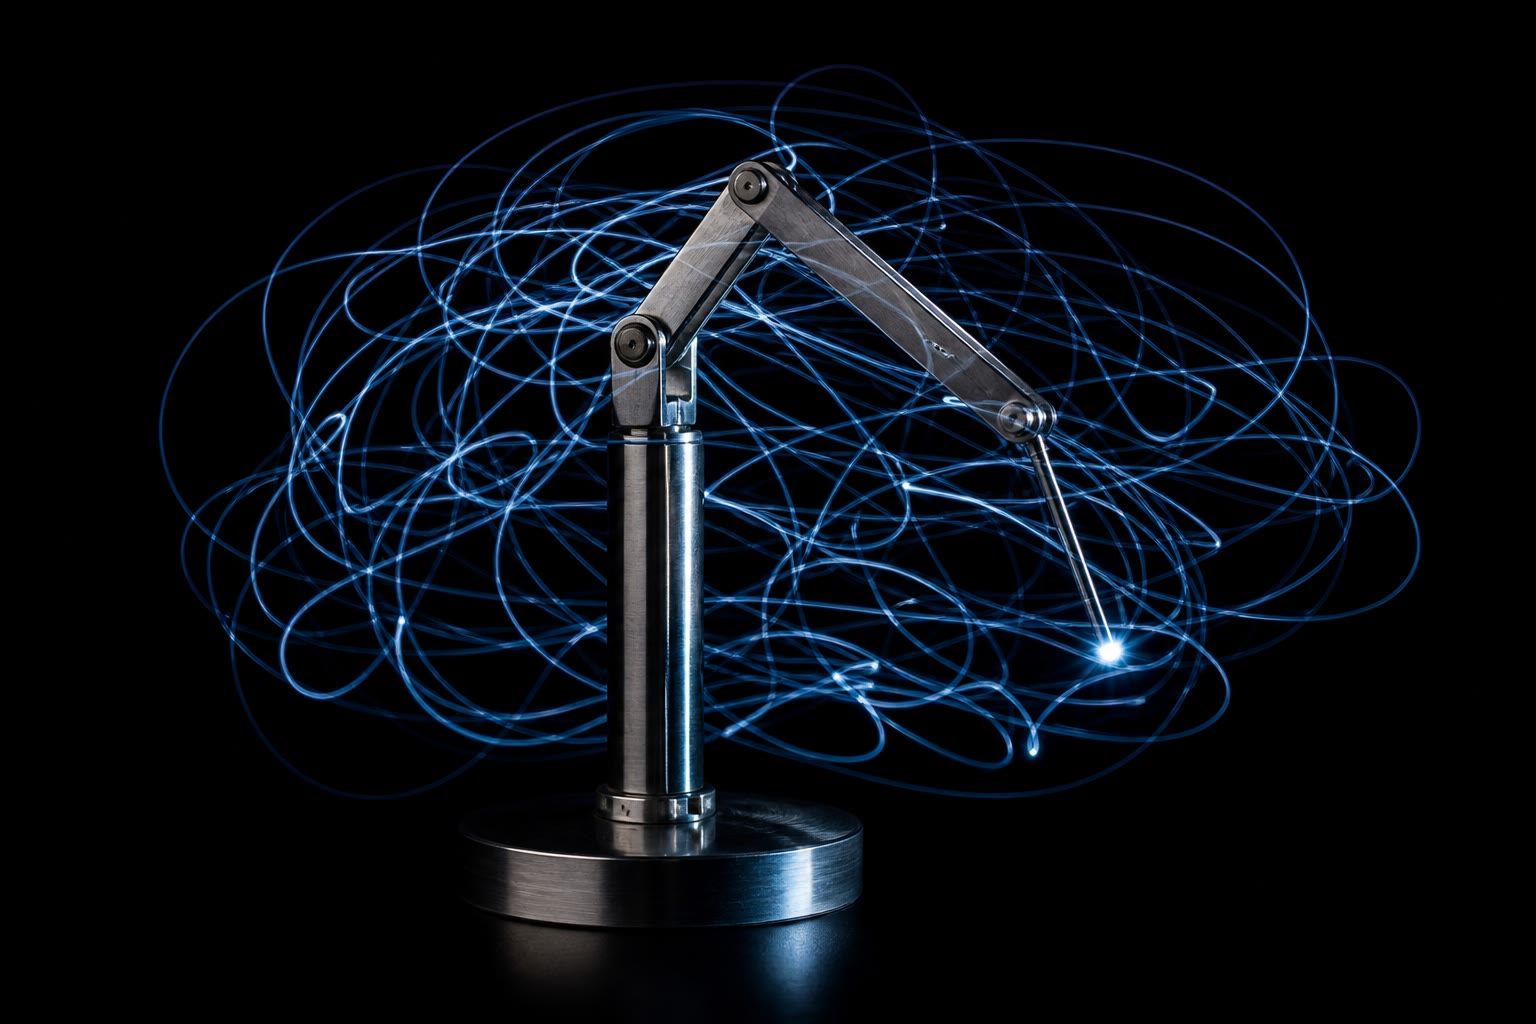
\includegraphics[width=0.58\linewidth]{images/book5/ai/b5-01-double-pendulum-trace.jpg}

{\small 长曝光记录下的双摆轨迹：两个坐标，一个拉格朗日量，以及一种长时间看来无法用公式预测的运动——本章的最小作用量机制写出了方程；混沌则让这些解保持谦逊。}
\end{omfigure}

\section{练习}

\begin{exercise}[$\star$]\label{exo:b3:lagrangian-mechanics:1}
数出自由度并提出广义坐标：（a）固定碗内侧的
质点；（b）沿固定斜面做无滑动滚动的
圆柱体；（c）上支点可在水平导轨上滑动的
双摆；（d）空间中的哑铃（两个质点、刚性细杆）；
（e）同一固定圆形金属丝上的两颗小珠。以上列表中
哪一个约束涉及的是速度而非位置，
它为何仍可积分为完整约束？
\end{exercise}

\begin{exercise}[$\star$]\label{exo:b3:lagrangian-mechanics:2}
对平面单摆（见\cref{ex:b3:lagrangian-mechanics:pendulum}）：
（a）验证 $L$ 与 $p_\theta =
\partial L/\partial\dot\theta$ 的量纲；（b）说明 $p_\theta$ 的物理意义；（c）
推出小角度下的周期；（d）计算一次完整微小振动的作用量 $S$，
其振幅为 $\theta_0$ ——并在计算前先说明结果
（简谐振动中 $E_k - E_p$ 的时间平均值
是多少？）
\end{exercise}

\begin{exercise}[$\star$]\label{exo:b3:lagrangian-mechanics:3}
阿特伍德机：质量分别为 $m_1$ 和 $m_2$ 的物体挂于理想绳两端，
绳跨过无质量的滑轮。（a）选取一个坐标并写出 $L$。（b）
求加速度。（c）牛顿的处理方法需要用到张力——
它去哪儿了？（d）运动一旦已知，
又该如何求出张力？
\end{exercise}

\begin{exercise}[$\star$]\label{exo:b3:lagrangian-mechanics:4}
柱坐标中的自由质点：$L = \tfrac12 m(\dot r^2 +
r^2\dot\varphi^2 + \dot z^2)$。（a）哪些坐标是循环的，并且
它们对应的守恒动量是什么？（b）为什么 $p_r$ \emph{不}守恒，
尽管没有力作用？（c）写出
$r$ 的欧拉–拉格朗日方程，并解释项 $mr\dot\varphi^2$ 的含义。（d）验证以恒定速率沿
直线运动的解满足该方程。
\end{exercise}

\begin{exercise}[$\star\star$]\label{exo:b3:lagrangian-mechanics:5}
质量为 $m$ 的物块沿楔块的无摩擦斜面（倾角 $\alpha$）滑动，
楔块质量为 $M$，本身可在无摩擦地面上滑动。（a）
选取两个坐标：楔块的横坐标 $X$ 与物块沿斜面向下的
距离 $s$；写出 $L$。（b）哪一个坐标是循环坐标，
它对应哪条守恒律？（c）求出两个
加速度。（d）检验极限 $M \to \infty$ 以及 $\alpha \to
90^\circ$ 的情形。
\end{exercise}

\begin{exercise}[$\star\star$]\label{exo:b3:lagrangian-mechanics:6}
球面摆：长为 $\ell$ 的杆末端悬挂一个摆锤，
两个角均可自由变化（$\theta$ 自竖直向下方向量起，$\varphi$ 为绕竖直方向的转角）。（a）
写出 $L$。（b）指出循环坐标及
其守恒量 $p_\varphi$。（c）将 $\theta$ 的运动化为有效势能问题，
并画出草图。（d）对圆锥运动 $\theta =
\theta_0$，导出圆锥摆关系式 $\cos\theta_0 =
g/\ell\omega^2$，该式见本科一年级分册。
\end{exercise}

\begin{exercise}[$\star\star$]\label{exo:b3:lagrangian-mechanics:7}
一个单摆（质量为 $m$，摆长为 $\ell$）挂在质量为 $M$ 的小车上，
小车可沿水平导轨自由滚动。（a）取坐标 $X$（小车）和
$\theta$，写出 $L$。（b）何量守恒？从物理上说为何守恒？（c）
在小 $\theta$ 下线性化，证明振动频率为
$\Omega = \sqrt{(1 + m/M)\,g/\ell}$。（d）解释极限 $M \to
\infty$ 与 $M \to 0$ 的情形——为何轻小车会\emph{提高}
频率？
\end{exercise}

\begin{exercise}[$\star\star$]\label{exo:b3:lagrangian-mechanics:8}
电荷为 $q$ 的质点处于均匀磁场 $\vect B = B\vect e_z$ 中，
其矢势为 $\vect A = \tfrac12\vect B\wedge\vect r$。（a）在直角坐标中写出 $L$。
（b）导出运动方程，并验证其描述的是
角频率为 $\omega_{\text{c}} = qB/m$ 的回旋圆运动。（c）
计算共轭动量 $p_x$、$p_y$：它们是否为 $m\dot x$、
$m\dot y$？它们是否守恒？（d）证明用柱坐标写出的 $L$
中 $\varphi$ 为循环坐标，并指出以轴为圆心的
圆周运动中的守恒量 $p_\varphi$。
\end{exercise}

\begin{exercise}[$\star\star$]\label{exo:b3:lagrangian-mechanics:9}
对于旋转圆环上的珠子
（见\cref{ex:b3:lagrangian-mechanics:hoop}）：（a）计算能量函数
$h$，并验证它在运动方程下守恒；（b）
计算机械能 $E$，并证明 $E - h =
m\omega^2R^2\sin^2\theta$；（c）求电动机输出的功率，表示为
$\theta$ 与 $\dot\theta$ 的函数；（d）求
当 $\omega^2 > g/R$ 时，倾斜平衡位置附近微小振动的频率，
并证明当 $\omega^2 \to g/R$ 时它趋于零 ——这种减慢
预示着势阱的分裂。
\end{exercise}

\begin{exercise}[$\star\star\star$]\label{exo:b3:lagrangian-mechanics:10}
等质量等长双摆（$m_1 = m_2 = m$，$\ell_1 = \ell_2 = \ell$）。
（a）证明在小角度下 $L = \tfrac12 m\ell^2(2\dot\theta_1^2 +
2\dot\theta_1\dot\theta_2 + \dot\theta_2^2) - \tfrac12 mg\ell(2
\theta_1^2 + \theta_2^2)$。（b）写出两个运动方程。（c）
求简正频率 $\Omega_\pm^2 = (2 \mp \sqrt2)\,g/\ell$，
以及各模式的形态（$\theta_2 = \pm\sqrt2\,\theta_1$）。（d）在大振幅下，
该系统是混沌的标准例子：用几句话解释
什么破坏了小角度分析，以及为何
并未丢失任何守恒律。
\end{exercise}

\begin{exercise}[$\star\star\star$]\label{exo:b3:lagrangian-mechanics:11}
\emph{最速降线。}一颗珠子无摩擦地从原点静止释放，
沿曲线 $y(x)$（$y$ 轴向下为正）滑到点 $(a, b)$。（a）
由能量守恒，证明下降时间为 $T =
\int_0^a\sqrt{(1 + y'^2)/2gy}\,\dd x$——一个泛函，其中 $x$
扮演时间的角色。（b）被积函数 $F(y, y')$ 不显含
$x$，证明 $h = y'\,\partial F/\partial y' - F$ 沿
最优曲线为常数（与
\cref{prop:b3:lagrangian-mechanics:energy}的计算相同）。（c）由此推出 $y(1 + y'^2) =
2r$，其中 $r$ 为常数，并验证摆线 $x = r(\phi -
\sin\phi)$，$y = r(1 - \cos\phi)$ 满足该式。（d）证明珠子沿
摆线一拱滑至底部所需时间为 $\pi\sqrt{r/g}$，并与
同一点处的直线滑道相比较。
\end{exercise}

\begin{exercise}[$\star\star\star$]\label{exo:b3:lagrangian-mechanics:12}
\emph{费马原理即最小作用量。}光在折射率为 $n(y)$ 的介质中，
沿两点间用时最短的路径传播（见本科二年级分册）。（a）证明
沿 $y(x)$ 的传播时间为 $T = \tfrac1c\int n(y)\sqrt{1 +
y'^2}\,\dd x$。（b）由于被积函数不显含 $x$，利用
上一题中守恒的 $h$，证明 $n(y)\big/\sqrt{1 +
y'^2} = \text{常数}$，并验证这即斯涅耳定律 $n\sin i =
\text{常数}$，其中光线的角度自竖直方向量起。（c）在炎热路面上方，
折射率随高度按 $n(y) \approx n_0(1 + \beta y)$ 增大；
证明近水平光线的弯曲半径为 $R \approx
1/\beta$。（d）取 $\beta = \qty{1.2e-5}{m^{-1}}$，
驾驶者双眼位于路面以上 \qty{1.2}{m} 处，问在距离多远时
能在路面上看到“水”状蜃景？
\end{exercise}

\begin{omfigure}
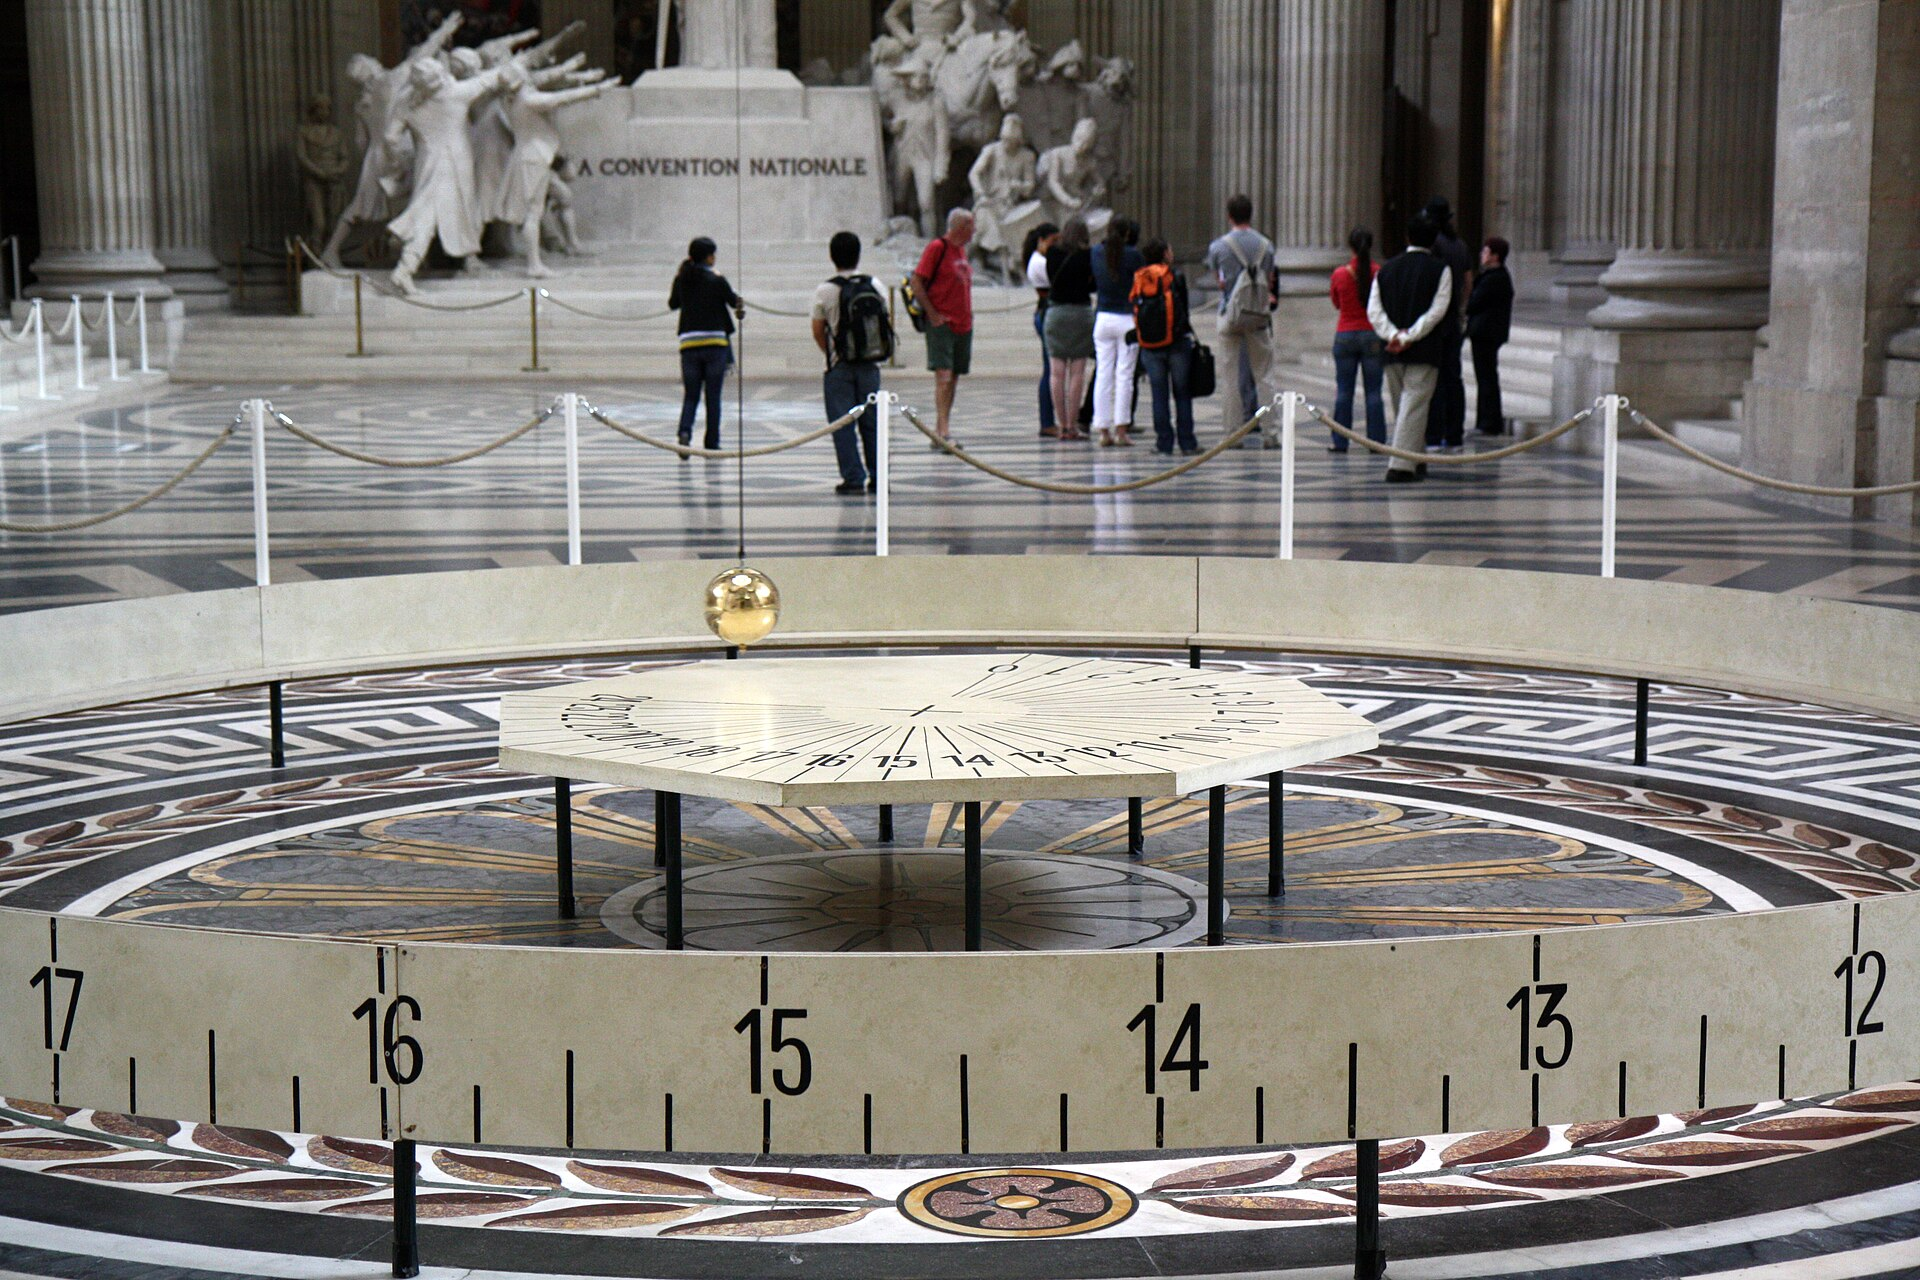
\includegraphics[width=0.6\linewidth]{images/book5/photo-foucault-pantheon.jpg}

{\small 傅科摆，位于巴黎先贤祠。广义坐标、约束，以及缓慢转动的参考系：房间的转动出现在运动方程中——而摆动平面的漂移使地下室得以测量地球的自转。照片：Olga Khomitsevich，CC~BY~2.0。}
\end{omfigure}

\section{问题：倒立的扫帚}

\begin{problem}[{周末问题——卡皮查的倒立摆}]\label{pb:b3:lagrangian-mechanics:1}
刚性摆若支点上下抖动得足够快，便能稳定地立于
其支点\emph{上方}——这一发现由卡皮查
于 1951 年分析，其效果几近魔术，其原理亦
可用于以振荡电场囚禁单个离子。我们将摆模型化为
一质点 $m$，位于一根无质量刚性杆的末端，
杆长 $\ell = \qty{40}{cm}$；$\theta$ 为自
\emph{竖直向下}方向量起的角度；$g = \qty{9.81}{m/s^2}$。

\medskip\noindent\textbf{第一部分——刚性摆。}
支点先保持固定。
\begin{enumerate}
  \item 写出拉格朗日量及运动方程。
  \item 给出小振动的频率 $f_0$（在 $\theta =
        0$ 附近），并求其数值。
  \item 证明此处 $h = E$，并利用其守恒求
        摆球在最低点应具有的最小发射速率，使其能够
        到达最高点。
  \item 在 $\theta = \pi$ 附近线性化方程（取 $\theta = \pi +
        \epsilon$），并证明 $\ddot\epsilon = +(g/\ell)\epsilon$：初始一毫度的倾斜
        会以多快的速度增长？给出
        其增长为原来 $e$ 倍所需的时间。
  \item 立于指尖的扫帚约一秒钟便倒下，然而
        它从不能独自直立：用一句话概括线性化方程
        对平衡 $\theta = \pi$ 所作的结论。
\end{enumerate}

\medskip\noindent\textbf{第二部分——支点的振动。}
支点现在竖直振动，其高度 $y_{\text{s}}(t) =
a\cos\Omega t$，其中 $a = \qty{2.0}{cm}$，$\Omega$ 可调。
\begin{enumerate}[resume]
  \item 写出摆球的坐标，并证明
        $\vect v^{\,2} = \ell^2\dot\theta^2 -
        2a\Omega\ell\sin(\Omega t)\sin\theta\,\dot\theta +
        a^2\Omega^2\sin^2\Omega t$。
  \item 证明两个相差一个全时间导数
        $\dd F(q,t)/\dd t$ 的拉格朗日量给出相同的欧拉–拉格朗日方程。
  \item 利用这一自由，将拉格朗日量化简为 $L = \tfrac12 m
        \ell^2\dot\theta^2 - ma\Omega^2\ell\cos(\Omega t)\cos\theta +
        mg\ell\cos\theta$。（提示：$\sin(\Omega t)\sin\theta\,\dot\theta$
        与一项 $\cos(\Omega t)\cos\theta$ 相合，构成全
        导数；仅含 $t$ 的项可略去。）
  \item 推导运动方程
        \[
        \ddot\theta = -\frac{g}{\ell}\sin\theta
         + \frac{a\Omega^2}{\ell}\cos(\Omega t)\sin\theta .
        \]
        将第二项理解为：重力被替换为 $g +
        \ddot y_{\text{s}}$：摆如同身处电梯之中。
  \item 现在能量函数 $h$ 是否守恒？能量是否守恒？
        是什么在输入和输出能量？
  \item 在卡皮查情形 $a \ll \ell$ 且 $\Omega \gg \omega_0 =
        \sqrt{g/\ell}$：校验这些条件，对 $a = \qty{2}{cm}$，$\ell =
        \qty{40}{cm}$，$\Omega/2\pi = \qty{40}{Hz}$，并
        从物理上解释为何此时摆球无法跟随驱动。
\end{enumerate}

\medskip\noindent\textbf{第三部分——快慢分离。}
试取 $\theta(t) = \Theta(t) + \xi(t)$：
即慢漂移 $\Theta$ 加上驱动频率下的小幅波动 $\xi$。
\begin{enumerate}[resume]
  \item 两边各仅保留最大项，证明波动
        满足 $\ddot\xi \approx +(a\Omega^2/\ell)\cos(\Omega t)
        \sin\Theta$，其中 $\Theta$ 在驱动时间尺度上视为不变。
  \item 由此推出 $\xi(t) = -(a/\ell)\cos(\Omega t)\sin\Theta$，并验证
        其振幅很小，量级为 $a/\ell$。
  \item 将 $\sin\theta = \sin(\Theta + \xi)$ 展开至
        $\xi$ 的一阶，并代入运动方程。
  \item 在一个驱动周期内取平均，其中 $\Theta$ 保持不变：
        利用 $\langle\cos\Omega t\rangle = 0$ 及
        $\langle\cos^2\Omega t\rangle = \tfrac12$，证明
        \[
        \ddot\Theta = -\frac{g}{\ell}\sin\Theta
         - \frac{a^2\Omega^2}{2\ell^2}\sin\Theta\cos\Theta .
        \]
  \item 证明这是在有效势能中的运动：
        \[
        U_{\text{eff}}(\Theta) = mg\ell\Big({-\cos\Theta}
         + \frac{a^2\Omega^2}{4g\ell}\sin^2\Theta\Big) .
        \]
  \item 与旋转圆环上的珠子作比较
        （见\cref{ex:b3:lagrangian-mechanics:hoop}）：数学形式相同，
        新增项符号相反——振动对旋转未能改变的
        \emph{底部}平衡点有何作用？
  \item 分别画出慢驱动与快驱动下的 $U_{\text{eff}}$ 示意图，并
        说明每种情形下各平衡点及其稳定性。
\end{enumerate}

\medskip\noindent\textbf{第四部分——扫帚竖立起来}
\begin{enumerate}[resume]
  \item 将 $U_{\text{eff}}$ 在 $\Theta = \pi$ 附近展开，证明
        倒立位置稳定当且仅当
        \[
        a^2\Omega^2 > 2g\ell .
        \]
  \item 对于我们的摆，计算临界驱动频率 $f_{\text{c}} =
        \Omega_{\text{c}}/2\pi$，以及它所需的支点峰值速率
        $a\Omega_{\text{c}}$ 和峰值加速度
        $a\Omega_{\text{c}}^2$（以 $g$ 为单位）。
  \item 取 $\Omega = 2\Omega_{\text{c}}$，求
        直立摆绕 $\Theta = \pi$ 缓慢摆动的频率，
        并给出其数值，验证它与驱动相比确实缓慢，
        即远小于驱动频率。
  \item 仍取 $\Omega = 2\Omega_{\text{c}}$，求波纹
        振幅 $\xi$ 在 $\Theta$ 略偏离 $\pi$ 处，以度计为多少？
        当 $a/\ell = 0.05$ 时，照片能否暴露这一把戏？
  \item 扫帚离竖直方向最多能倾斜多远仍能回到直立？
        证明直立区域延伸至 $|\Theta - \pi| <
        \arccos(2g\ell/a^2\Omega^2)$，并在 $\Omega =
        2\Omega_{\text{c}}$ 处计算其值。
  \item 杂技演员在静止的指尖上平衡扫帚，也能使其竖立——
        依靠的是何种完全不同的机制？请指出
        卡皮查摆中无需反馈的那一特征。
  \item 总结这一著名结论：支点以振幅
        \qty{2}{cm}、频率 \qty{45}{Hz} 振动，恰为临界频率的两倍——
        可使 \qty{40}{cm} 的摆倒置保持，
        其势阱延伸至偏离竖直方向约 $75^\circ$ 处，并以
        约 \qty{1.4}{Hz} 的频率轻柔摆动。物理学中，何处用同样的平均
        束缚手段囚禁单个带电粒子？
\end{enumerate}
\end{problem}
